% !TeX root = ../../main.tex
% Add the above to each chapter to make compiling the PDF easier in some editors.

\section{Inside-Outside Guidance}\label{ord:ch3:sec4}

Another approach for interactive segmentation is the \gls{iog} method, introduced in \cite{Zha20-IOG}.
The concept of this state-of-the-art method relies on user points and \gls{dl} (see Section \ref{ord:ch2:sec3:subsec2}. 

\subsection{Basis Concept}\label{ord:ch3:sec4:subsec1}
% User Clicks - Workflow
The user interaction of the \gls{iog} method requires three user clicks executed in two steps.
First, the user has to draw a tight bounding box around the object of interest. 
The drawing of the bounding box is normally counted as two user clicks on the background.
% TODO refine the stroke possibility
%The creation of the bounding box is implemented using a stroke instead of setting two clicks.
Second, the user has to click once on the center of the object, which is represented as foreground click. 
This described workflow is illustraded in Figure \ref{fig:ch3:sec4:iog_user_clicks}
Further, the user clicks are processed and an object mask is predicted by a \gls{dl} model.

% Naming of the method
% two-fold
The user provides high level guidance on the foreground and background, representative on the inside and outside region of the object.
On the one hand, this guidance is based on the bounding box that defines the background.
So, everything outside the bounding box does not belong to the object, this is described as \textit{outside} guidance.
On the other hand, the foreground click provides explicit guidance, where the object is located.
This is referred to as \textit{inside} guidance.
These two types of guidance are the namesake of the method \glsentryfull{iog}.

% Advantage over DEXTR
Zhang claims that her way to set user clicks has two advantges over the way to set user clicks in other interactive methods as \gls{dextr}.
First, the setting of extreme points may be confusig and misleading, as they may be located very close to each other, depending on the object's orientation.
Second, if the obejct of interst contains a hole (\ie a donut) or is in the background of another object, \gls{dextr} cannot provide a robust guidance.
In contrast, the variable position of the foreground click in \gls{iog} enables a more robust guidance even for special object scenarios.

\begin{figure}
	\centering
	\begin{subfigure}[b]{0.3\textwidth}
		\centering
		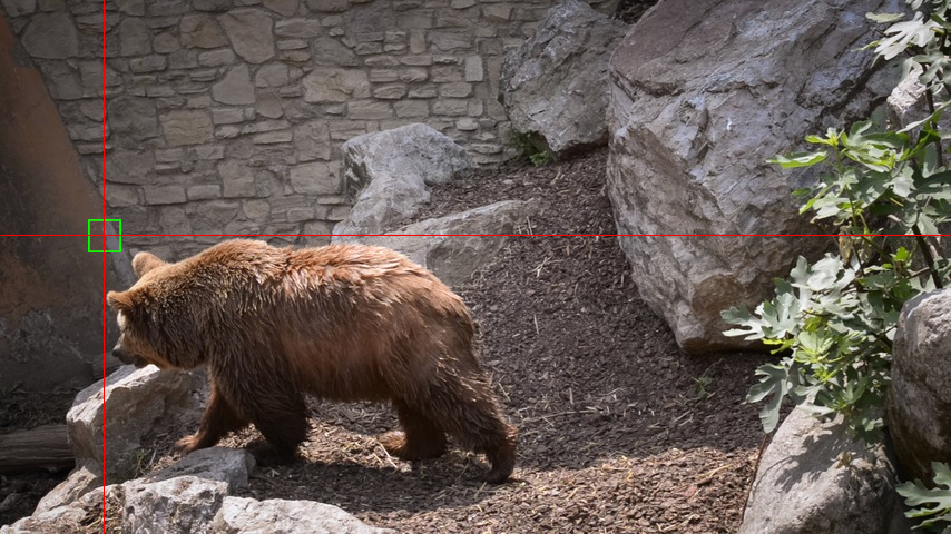
\includegraphics[width=\textwidth]{figures/chap34_bear_2.png}
		\caption{First background click.}
		\label{fig:ch3:sec4:iog_workflow_1}
	\end{subfigure}
	\hfill
	\begin{subfigure}[b]{0.3\textwidth}
		\centering
		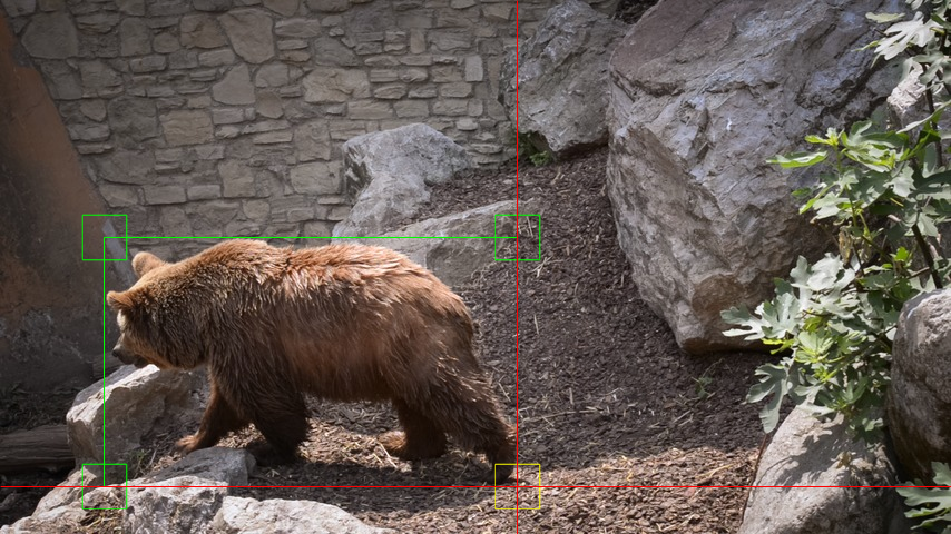
\includegraphics[width=\textwidth]{figures/chap34_bear_3.png}
		\caption{Second background click.}
		\label{fig:ch3:sec4:iog_workflow_2}
	\end{subfigure}
	\hfill
	\begin{subfigure}[b]{0.3\textwidth}
		\centering
		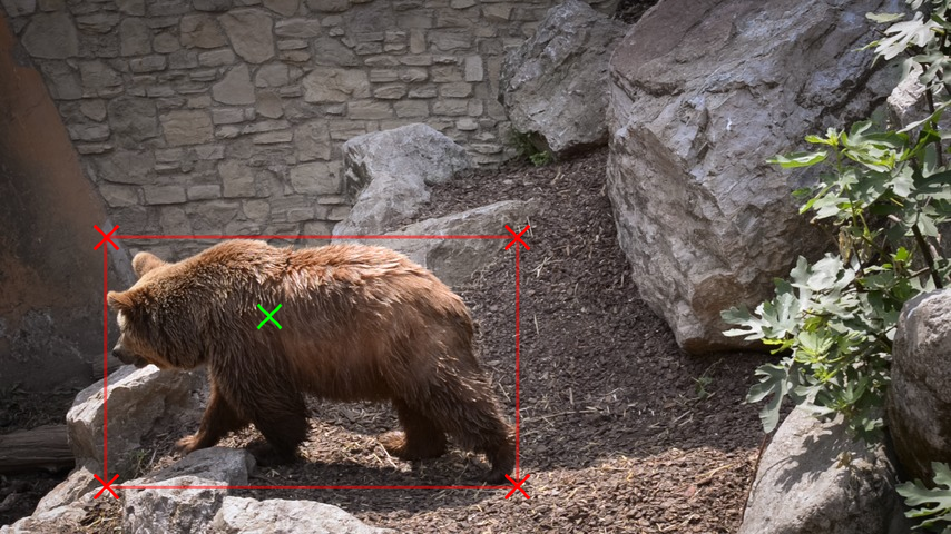
\includegraphics[width=\textwidth]{figures/chap34_bear_5.png}
		\caption{Foreground click.}
		\label{fig:ch3:sec4:iog_workflow_3}
	\end{subfigure}
	\caption[IOG Application]{
		Shown is the workflow to perform the user interaction required for the \gls{iog} method.
		First, a bounding box is spanned by setting two background clicks.
		Last, the foreground click is set.
		All available points are visualized with a cross, background points in red and the foreground point in green, while the contour of the bounding box is drawn in red.
	} 
	\label{fig:ch3:sec4:iog_user_clicks}
\end{figure}

\subsection{Representation of User Clicks and Model Input}\label{ord:ch3:sec4:subsec2}

The bounding box is set by the two diagonal corners points (top-left and bottom-right or bottom-left and top-right).
Based on these two points, the other two corner points are derived, which provides four background points to the price of two.
Further the bounding box is enlarged by $p_{{box}}$ pixels to include context from the surrounding region and ensure no background point is set on the edge of the object.
%TODO use parameter later to describe my experimental setup.

In order to focus on the object of interest, the image is cropped based on the enlarged bounding box.
The crop is resized to the size of $512 \times 512$ \Unit{px}. 
The fore and background clicks are converted into points on two separate heatmaps.
To highlight the user points a 2D Gaussian is centered around each click, as in the \gls{dextr} method.
The two heatmaps have the size of $512 \times 512$ \Unit{px} and are concatenated with the RGB image.
For the model this results into a five-channel input, which is explanatory illustrated in Figure \ref{fig:ch3:sec4:model_input_channels}.

\begin{figure}
	\centering
	\begin{subfigure}[b]{0.3\textwidth}
		\centering
		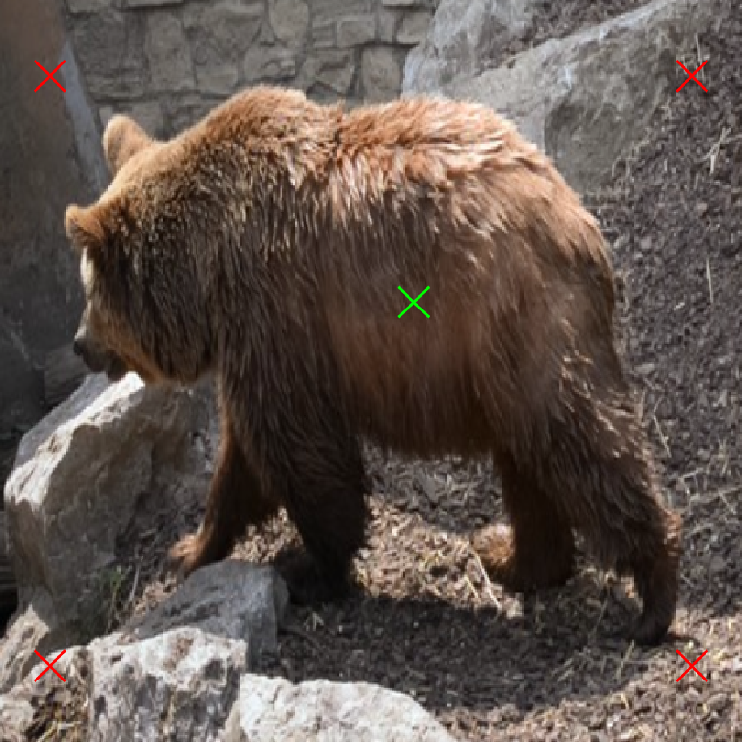
\includegraphics[width=\textwidth]{figures/chap34_channel_rgb.png}
		\caption{RGB image cropped based on the bounding box (three channels).}
		\label{fig:ch3:sec4:rgb_channel}
	\end{subfigure}
	\hfill
	\begin{subfigure}[b]{0.3\textwidth}
		\centering
		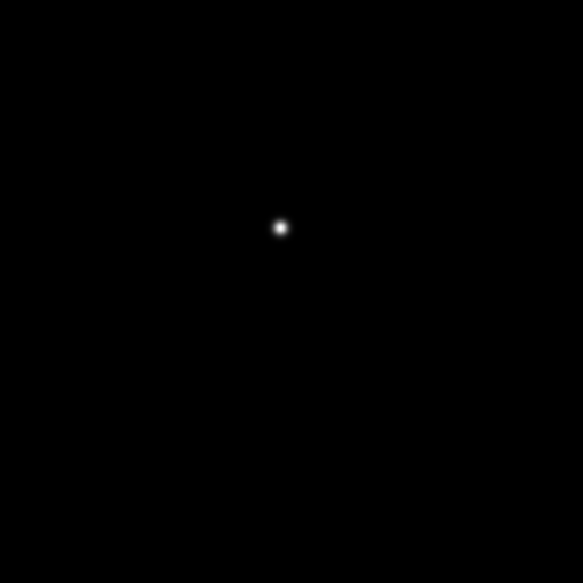
\includegraphics[width=\textwidth]{figures/chap34_channel_fg.png}
		\caption{Foreground heatmap with one foreground point (one channel).}
		\label{fig:ch3:sec4:fg_channel}
	\end{subfigure}
	\hfill
	\begin{subfigure}[b]{0.3\textwidth}
		\centering
		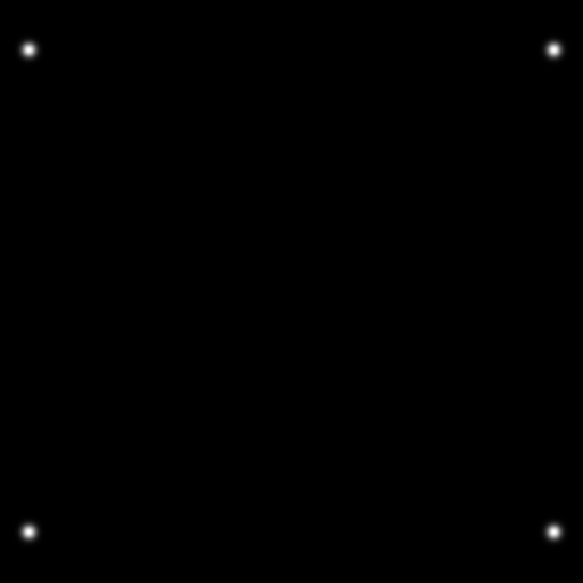
\includegraphics[width=\textwidth]{figures/chap34_channel_bg.png}
		\caption{Background heatmap with four background points (one channel).}
		\label{fig:ch3:sec4:bg_channel}
	\end{subfigure}
	\caption[Five-channel IOG model input]{
		Separate channel representation of the five-channel \gls{iog} model input.
		All channels have the spacial dimension of $512 \times 512$ \Unit{px}.
		The user points in the foreground and background are enforced with a 2D Gaussian.
	} \label{fig:ch3:sec4:model_input_channels}
\end{figure}

\subsection{Architecture}\label{ord:ch3:sec4:subsec3}

The model architecture used for the \gls{iog} method is based on the encoder-decoder architecture and special structure for layer fusion.
The encoder-decoder network is titled as \textit{CoraseNet}, while the structure for layer fusion is referred to as \textit{FineNet}.
An illustration of the complete architecture is given in Figure \ref{fig:ch3:sec4:arch}.


\subsubsection{CoarseNet}
The CoarseNet consists out of multiple components: encoder network, decoder network, \gls{psp}-module and skip connections. The CoarseNet is built upon the \gls{dextr} method, therefore they partially share the same architectural components. 
% TODO write DEXTR Architecture -> are just the first components of the corase net the same in DEXTR?

For the encoder network a ResNet-101 \cite{He16-ResNet} is used, also referred to as backbone.
%The ResNet is implemented without the head of fully connected layers. It contains four ResNet blocks and the fourth block outputs 2048 feature maps of the size $32 \times 32$ \Unit{px}.
As in \gls{dextr} a \gls{psp}-module is applied after the backbone to gain more contextual information.
The output of the \gls{psp}-module is a coarse prediction with the spatial dimension of  $32 \times 32$ \Unit{px} containing 512 feature maps. 

From this onward the decoder network starts the upsampling process. 
The spatial dimension of the feature maps are enlarged in four stages, in order to regain the original input size of  $512 \times 512$ \Unit{px}. 
In the upsampling process skip connection are applied to each stage.
The skip connections originate from corresponding residual part of the backbone.
% TODO this skip connection also does some processing
% During the upsampling process activations from the residual blocks of the ResNet are transferred from the ResNet using so lateral connections and concatenated with the upsampled feature maps.
% A benefit of this architecture is the fusion of information from different network stages.
\begin{figure}
	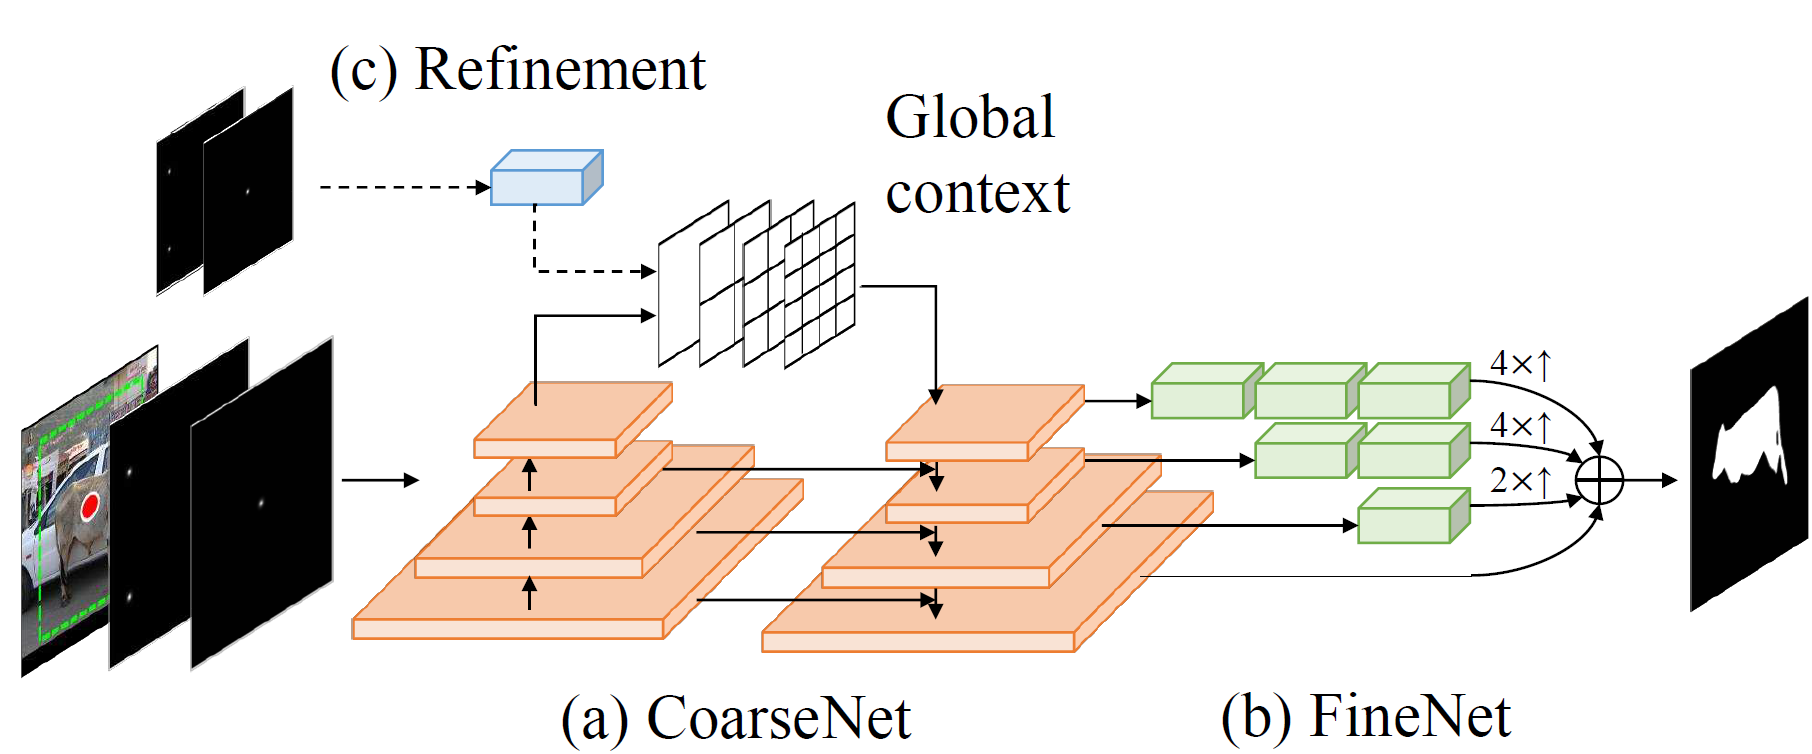
\includegraphics[width=\linewidth]{figures/chap34_iog_arch.png}
	\caption[IOG Architecture]{		
		Architecture of the \gls{iog} model.
		On the left the model input is visualized as in Figure \ref{fig:ch3:sec4:model_input_channels}.
		The CoarseNet is marked by (a) and shows the encoder and decoder network with the lateral skip connections and the \gls{psp} module.
		The FineNet is marked by (b) and represents the four stream fusion structure.
		It can be seen, that the single streams origin from different levels of the decoder network.
		Therefore, each stream applies different processing and upsampling, in order to obtain the same spatial dimension for concatenation.		
		As final prediction a binary object mask is shown.
		The \textit{lightweight-branch} for refinement is marked with (c).
		Copyright \copyright 2020 IEEE. Reprinted by permission from \cite{Zha20-IOG}.
	}
	\label{fig:ch3:sec4:arch}
\end{figure}

\subsubsection{FineNet}
The FineNet represents a four-stream fusion structure.
The four streams originate from the four levels of the decoder network and therefore face feature maps of various sizes (see Figure \ref{fig:ch3:sec4:arch}).
Each stream processes and upsamples the feature maps by a descending number of bottleneck processing blocks.
The streams reconstruct the feature maps to the final spatial dimension of $512 \times 512$ \Unit{px}.
%applied in order to use \emph{"features at deeper layers for better trade-off between accuracy and efficiency"} \cite[p. 12237]{Zha20-IOG}.
In the end the four streams are concatenated and pass through a final bottleneck processing block.
To the final output a sigmoid is applied, which results in a probability map as final prediction of the \gls{iog} network.

The author justifies the application of these different components by showing their effect in an ablation study \cite{Zha20-IOG}.
% The author shows in an ablation study, that the FineNet enhances the networks IoU by $0.8\%$. 
% The ablation study is performed with a ResNet-50 as backbone and PASCAL-1k \cite{Eve20-PascalVOC} as dataset. 


\subsection{Refinement}\label{ord:ch3:sec4:subsec4}

As introduced in Subsection \ref{ord:ch2:sec3:subsec2}, some methods provide the possibility to perform refinement, if a segmentation results does not meet the user's expectations.
To perform refinement in the \gls{iog} method, the user sets an additional click on the fore- or background region with the greatest error.
Each refinement clicks triggers a new model execution.
The refinement process may be applied iteratively.

The integration in the existing architecture is realized as the following.
New heatmaps for fore- and background are created with the original clicks and the refinement clicks.
These two heatmaps are combined into a two-channel input, which is processed in a so called \textit{lightweight-branch}.
This lightweight-branch consists out of five convolutional layers, that perform the downsampling.
The output of this branch is combined with the output of the encoder network's initial iteration and forwarded to the \gls{psp} module as shown in Figure \ref{fig:ch3:sec4:arch}.
From the \gls{psp} module on the model is executed normally.

Hence, the encoder network does not require a new execution, the model's execution time is decreased as well.
Zhang states, that the usage of the lightweight-branch performs better, than directly adding the refinement click into the normal five-channel input.

\begin{figure} 
	\centering
	\begin{subfigure}[b]{0.45\textwidth}
		\centering
		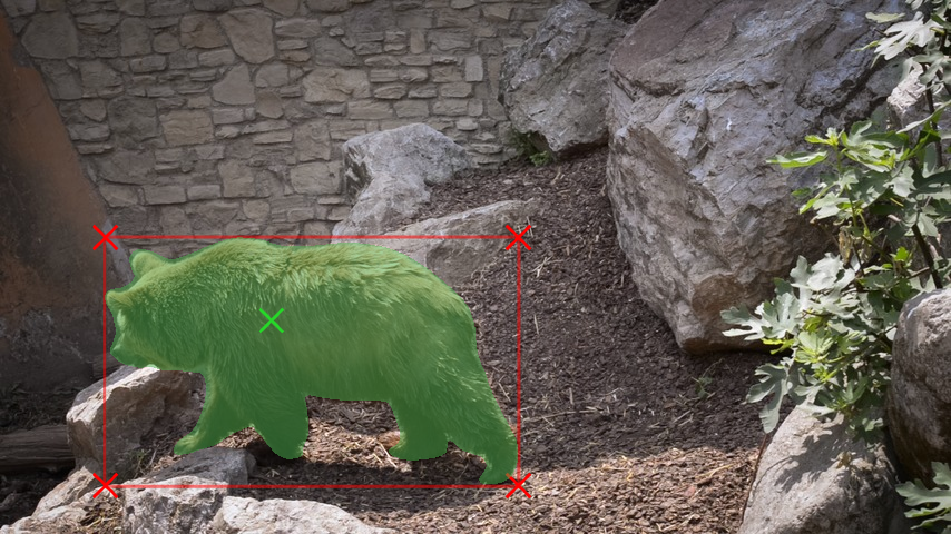
\includegraphics[width=\textwidth]{figures/chap34_bear_6.png}
		\caption{Initial segmentation result.}
		\label{fig:ch3:sec4:refinement_1}
	\end{subfigure}
	\hfill
	\begin{subfigure}[b]{0.45\textwidth}
		\centering
		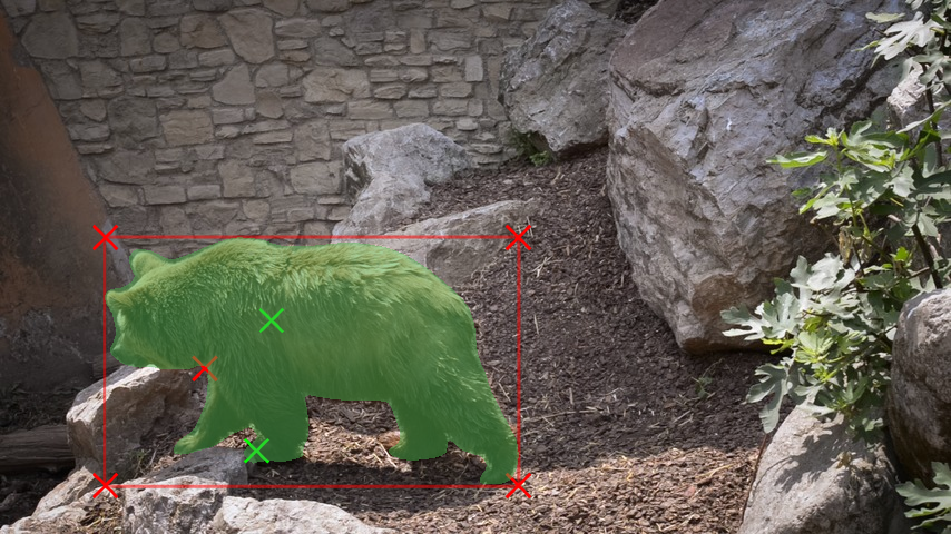
\includegraphics[width=\textwidth]{figures/chap34_bear_8.png}
		\caption{Refinement segmentation result.}
		\label{fig:ch3:sec4:refinement_2}
	\end{subfigure}
	\caption[IOG Refinement]{
		On the left is the initial result with the normal amount of clicks. 
		On the right is the results of two refinement iterations with one additional refinement clicks on the foreground and one on the background.
	} \label{fig:ch3:sec4:refinement}
\end{figure}


\subsection{Performance}\label{ord:ch3:sec4:subsec5}

An overview of interactive segmentation methods is shown in Table \ref{tab:ch2:interactive-stae-of-the-art}.
It can be seen that the \gls{iog} outperforms other state-of-the-art methods the number of set points and the achieved \gls{iog} at four clicks.

This method especially performs well due it's  architecture.
The application of skip connections and the FineNet enable the model to recover local details and prevent the information loss during down- and upsampling process.

In their experiments Zhang investigates the performance on unseen classes and the method's generalization capability \Cite{Zha20-IOG}.
Thereby, the model was trained with the Pascal VOC or COCO dataset and evaluated on both datasets.
Despite these results seem reliable, it must be taken into account that the Pascal VOC and COCO datasets are very similar and cover the same type of \textit{general} objects.
Further, Zhang also evaluated the performance on dataset of other domains (\eg CityScapes, Rooftops or Agricultural-Vision).
The \gls{iog} method trained on Pascal VOC outperformed the \gls{dextr} method or the \textit{Curve-\gls{gcn}}, both trained on the CityScapes dataset.
A detailed evaluation of the \gls{iog} and \gls{dextr} method is presented in Chapter XXX. 
%TODO ref -> evaluation chapter.
